%%「論文」,「レター」,「レター(C分冊)」,「技術研究報告」などのテンプレート
%% 1. 「論文」
%% v3.0 [2015/11/14]

%% 4. 「技術研究報告」
\documentclass[technicalreport]{ieicej}
%\usepackage[dvips]{graphicx}
%\usepackage[dvipdfmx]{graphicx,xcolor}
\usepackage[T1]{fontenc}
\usepackage{lmodern}
\usepackage{textcomp}
\usepackage{latexsym}
\usepackage[dvipdfmx]{graphicx}
\usepackage{graphicx}
\usepackage{amsmath}
\usepackage{txfonts}
\usepackage{url}
\usepackage{enumerate}
%\usepackage[fleqn]{amsmath}
%\usepackage{amssymb}

\setcounter{page}{1}

\jtitle{複数人で使用可能な3Dアイデアノートシステムの提案と実装}
\jsubtitle{}
\etitle{}
\esubtitle{}
\authorlist{%
 \authorentry{猪膝 孝之}{Takayuki INOHIZA}{uec}\MembershipNumber{uec}
 \authorentry{田野 俊一}{Shun'ichi TANO}{uec}\MembershipNumber{uec}
 \authorentry{橋山 智訓}{Tomonori HASHIYAMA}{uec}\MembershipNumber{uec}
 \authorentry{丸谷 大樹}{Taiki MARUYA}{uec}\MembershipNumber{uec}
 \authorentry{市野 順子}{Junko ICHINO}{tcu}\MembershipNumber{tcu}
 \authorentry{森 真吾}{Shingo MORI}{tis}\MembershipNumber{tis}
 \authorentry{井出 将弘}{Masahiro IDE}{tis}\MembershipNumber{tis}
% \authorentry[メールアドレス]{和文著者名}{英文著者名}{所属ラベル}
}
\affiliate[uec]{電気通信大学大学院 情報理工学研究科}{Graduate School of Informatics and Engineering, The University of Electro-Communications}
\affiliate[tcu]{東京都市大学 メディア情報学部}{Faculty of Informatics, Tokyo City University}
\affiliate[tis]{TIS株式会社}{TIS Inc.}
%\affiliate[所属ラベル]{和文勤務先\\ 連絡先住所}{英文勤務先\\ 英文連絡先住所}

\begin{document}
\begin{jabstract}
%和文あらまし
近年、HMD(Head Mounted Display) が普及してきた。現在、HMDに関する研究は一人で使用することを想定していたり、特定の場所で使用することを想定していたり、手やペンで描くのみで入力手法が限定されているものが多い。これらの問題点を踏まえた上で本研究では、複数人で使用可能で、どこでも場所を選ばず利用が可能で、直感的で様々な入力が可能なHMDを使用したシステムの提案を行う。これらのコンセプトに基づいたシステムを設計し、実際にプロトタイプシステムの実装を行った。また、評価実験ではシナリオ実験と課題解決実験の二つを行い、シナリオ実験での手順の遂行状況においてはほとんどの手順において成功率100\%を収めた。課題解決実験においても多くの被験者がタスクを実行できることが確認できた。
\end{jabstract}
\begin{jkeyword}
%和文キーワード
3D, メモ, 共有, マルチモーダル
\end{jkeyword}
%\begin{eabstract}
%英文アブストラクト
%\end{eabstract}
%\begin{ekeyword}
%英文キーワード
%\end{ekeyword}
\maketitle

\section{はじめに}
アイデアはふとしたときに思い浮かぶことがあり、私達はそれを紙に書き留めたり、PCやスマートフォン等を利用してメモを取ることがある。しかし、アイデアが思い浮かぶのは座って作業しているときだけでなく、外で歩いているときや、机やホワイトボード等がないような場面でも突然思い浮かぶことがある。紙とペンを持ち歩いて思い浮かんだらすぐにメモを取る習慣ができてる人はいいが、そうでない人はアイデアが思い浮かんでも「後でメモをすればいいや」と思ってすぐにメモを取ることを諦めてしまうだろう。実際に日頃からアイデアをメモに記録している人は少なくなってきている傾向がある。思い浮かんだアイデアはできるだけ早くメモを取ったほうが良い。また、アイデアは一人で考えて生み出すものとは限らない。友人との話し合いをしているうちに一人では思いつかなかったアイデアが生まれたり、話が弾んで連鎖的にアイデアが生まれることもある。アイデアを効率的に生み出すための発想法がすでに何種類もあるが、これらの中には複数人で集まって話し合ってアイデアを出すものも多い。

近年、HMD(Head Mounted Display)が普及してきた。HMDに関する研究はすでに多く行われている。医療技術に関する研究や、デザイナー向けの3Dスケッチに関する研究、他には3D空間上に文字や図形を描いたりする研究等もある。近年ではMRも流行化してきており、医療診断・手術計画や屋内外の誘導・案内、埋蔵物確認、都市計画・建築分野でのシミュレーション、アミューズメント産業等の応用分野から大きな期待がされている。

現在、HMDに関する多くの研究は一人で使うことが想定されている。また、特定の場所において使用することを想定している場合も多い。そして、手やペンで描くのみで入力手法が限定されている場合も多い。現状では複数人で使用することを想定していたり、外などの広い空間で利用することを想定していたり、手で描くだけでなく音声でも入力可能なシステムを想定している研究やアプリケーションは少ない。そこで、複数人で使用できて、どこでも利用できて、様々な入力ができるシステムが必要だと考え、本研究の立案に至った。

\section{従来研究と問題点}
椎尾らは仮想の手書きメモによるコミュニケーションをウェアラブルコンピュータにより実現する空気ペンを試作した。問題点としては、同時に複数人で使用できないことや、使用できる範囲がRFIDタグがついた床上のみなので場所が限定されることが挙げられる。

また、高山らは実世界のどのような時間・場所であっても、ユーザが思い浮かんだふとしたアイデアを、生起を誘発したコンテキストに対応づけて保存し、それを他のユーザと共有できるシステムを作成した。問題点としては、多くの機器を装着しなければならないので持ち運びが大変であることや、操作が複雑なので慣れるのに時間がかかることが挙げられる。

長田らはスマートグラスを用いた仮想空間への手書き情報共有システムを提案した。問題点としては、指のみの操作だとできることが限定されることが挙げられる。

従来研究のHMDを使用したシステムの問題点をまとめると以下である。

\begin{itemize}
 \item 同時に複数人で使用することを想定していない
 \item 利用できる場所が限定されている
 \item 入力手法が限定されている
\end{itemize}

\section{本研究のコンセプト}
従来研究のHMDを使用したシステムでは同時に複数人で使用することを想定していない、利用できる場所が限定されている、入力手法が限定されているという問題点があった。

そこで、従来研究の問題点を踏まえ、本研究は以下の三つを満たすようなHMDを使用したシステムを提案する(図\ref{fig:concept})。

\begin{enumerate}
 \item 複数人で同時に使用することが可能
 \item どこでも場所を選ばず利用が可能
 \item 簡単な操作で直感的で様々な入力が可能
\end{enumerate}

\begin{figure}[h]
  \begin{center}
    \includegraphics[clip,height=6.0cm,width=7.0cm]{./concept.eps}
    \caption{システムコンセプト}
    \label{fig:concept}
  \end{center}
\end{figure}

\subsection*{特徴1:複数人で同時に使用することが可能}
既存の研究では一人で使用することを想定したシステムが多かった。または、将来的には複数人で使用できるようにすることを目標にしてるが現状のシステムでは一人でしか使用できないというものも多かった。他には、複数人で使用することはできるが同時に使用することができないというものあった。アイデアは一人で考えて生み出す場合もあるが、複数人で集まって話し合って一緒に考えることによってアイデアが生まれることもある。ある人がアイデアを出せば、そのアイデアに対して他の人が反応して新たな意見を出して、そこからまた新しいアイデアが生まれることもある。それが連鎖的に続くことによって結果的にアイデアをたくさん生み出すことに繋がる。アイデアを効率的に生み出す方法が既に何種類も存在するが、その中には実際に複数人で集まって話し合ってアイデアを出し合うというものも多い。したがって、複数人で同時に使用できて、お互いのメモをリアルタイムで共有できることが必要不可欠である。また、複数人で利用する際に空間上に文字を残す場合に問題点が発生する。その問題点については\ref{moji_mondai}節で詳しく述べる。

\subsection*{特徴2:どこでも場所を選ばず利用が可能}
既存の研究では机やPCの近く、または特定の場所等のみでしか使用できないシステムが多かった。他には、どこでも利用可能ではあるが多くの機器を装着しなければならなかったり等、可搬性に問題があるシステムもあった。アイデアが生まれるのは椅子に座って机で作業しているときや、黒板やホワイトボードの前に立っているとき等、何かノート等を使ってメモを取ることができる場所だけとは限らない。アイデアは思いがけない場所でふとしたときに突然思い浮かぶことがある。時には外で歩いているときや、軽い運動をしているときに思い浮かぶこともある。実際に動きながらメモを取るのは困難である。また、普段から常にメモ帳等を持っていてすぐにメモを取る習慣がついている人は良いが、そうでない人はメモを取ることを諦めてしまったり、後回しにしまいがちである。アイデアが思い浮かんだら、当然すぐにメモを取るほうが良い。したがって、どこでも場所を選ばずに利用できるようなシステムが必要である。

\subsection*{特徴3:簡単な操作で直感的で様々な入力が可能}
既存の研究では空間上で描くのみ等で入力手法が限定されているシステムが多かった。または、特別なジェスチャを定義して使用する必要があったり、慣れるのにかなり時間がかかる等のシステムもあった。アイデアの形は文字や図形等、様々な形をとる。立体的な形を持ったアイデアもあれば、平面の形を持ったアイデアも存在する。仮に入力手法を空間上に描くのみにした場合、考えたアイデアが短い文章にまとまらないときメモを取ることが困難である。また、仮に入力手法を音声のみにした場合、シンプルな図形であれば表示できるかもしれないが、大きさを音声入力で指定しなければならなかったり、複雑な図形を描く際は困難である。したがって、簡単な操作で直感的で様々な入力ができるシステムが必要である。

\subsection{文字を表示する上での問題点と解決案} \label{moji_mondai}
複数人で空間上に文字のメモを残す際に、見る視点によって文字として見えないという問題点が発生する。解決案として、文字を動的に相手の方向に回転させて向けたり、文字のメモに触れたら自分の前に見えるように表示する等の方法が考えられる。しかし、文字を動的に相手の方向に回転させて向けてはいけない場合もある。それは、平面上に文字のメモを残した場合である。何故ならばその平面そのものに意味があるからである。このようなメモの表示に関しての解決案は、その平面上に残した文字のメモに目線を合わせて、それ自体はそのままにしておき、その平面上に残した文字を目の前等の自分の見やすい位置に表示するという手法を提案する。

また、平面の形を持った文字以外に立体的な形を持つ文字が存在すると考えられる。立体的な文字に関してはそれ自体に意味を持つので回転したり等はしないほうがよいと考えられる。

\section{システム設計}
本研究のコンセプトで述べたシステムコンセプト(1)、(2)、(3)を踏まえた上でシステムの全体構成について述べる。その次にそれぞれの機能の設計に関して詳しく説明する。また、ハードウェアは可搬性を考慮して、マイクロソフト社のHoloLensを使用する。

\subsection{全体構成}
(1)複数人で同時に話し合って使用できてお互いのメモを共有できるようにするために、サーバを介して空間を共有する機能が必要である。(2)どこでも場所を選ばずに利用できて、実世界の広い空間上に任意の場所にメモを置く際には、遠くにあるメモに対して操作する機能が必要である。また、(3)簡単な操作で直感的で様々な入力を可能にするには、3D空間上に描画する機能だけではなく、音声でも入力ができることが必要である。以上より、システムの機能としては大きく分けて、メモを入力、メモを操作、メモを共有の三つであり、以下に詳細を述べる。

\subsection{メモを入力}
実世界の任意の3D空間上に図形や文字のメモを描いて残したり話して残したりできるようにする。3D空間上に文字によるメモを相手に見えるようにするためには回転して相手に向けるという手法が考えられる。しかし、平面に残したメモの場合、その面自体に意味があるので回転させてはならない。そこで、正面からメモを見た場合はそのまま表示し、ある程度横から見た場合にはそのメモ自体はそのままだが、内容がわかるように目の前に見やすく表示をするという手法を提案する。(図\ref{fig:memo_wall})

\begin{figure}[h]
  \begin{center}
    \includegraphics[clip,height=6.0cm,width=4.0cm]{./memo_wall.eps}
    \caption{ある程度横から見た場合は目の前にも表示}
    \label{fig:memo_wall}
  \end{center}
\end{figure}

\subsection{メモを操作}
広い空間上にメモを残す場合、遠くに配置してあるメモをどうやって選択、移動、削除するかという問題が発生する。そこで、以下の三つのインタラクションを提案する。

\begin{enumerate}[(1)]
 \item ルームスケールチェンジ
 \item 3Dラバーバンド
 \item 3Dフィッシング
\end{enumerate}

(1)手元に部屋全体を縮小したものを用意してメモを操作する手法で、(2)はイメージとしては手元に輪ゴムがついたオブジェクトを引っ張って遠隔のメモを操作する手法、(3)は視線と手元のオブジェクトを利用して釣りのように遠隔のメモを操作する手法である。

\subsection{メモを共有}
実世界の任意の3D空間上に残したメモを対面にいる人だけでなく、遠隔にいる人にもメモを共有できるようにする。遠隔にいる人はアバターを実世界に表示させる。

\section{プロトタイプシステムの実装}
設計したシステムを基に行ったプロトタイプシステムの実装について述べる。

\subsection{プロトタイプシステムの構成}
設計されたシステムは、ユーザがシステムの各機能を利用するために使うアプリケーションと、HoloLens同士で相互接続するためのサーバ、ユーザが喋った内容をテキストに変換するクラウドサービスが存在する。図\ref{fig:prototypesystem1}にプロトタイプシステムの全体図を示す。以下でそれぞれについて述べる。

\begin{figure}[h]
  \begin{center}
    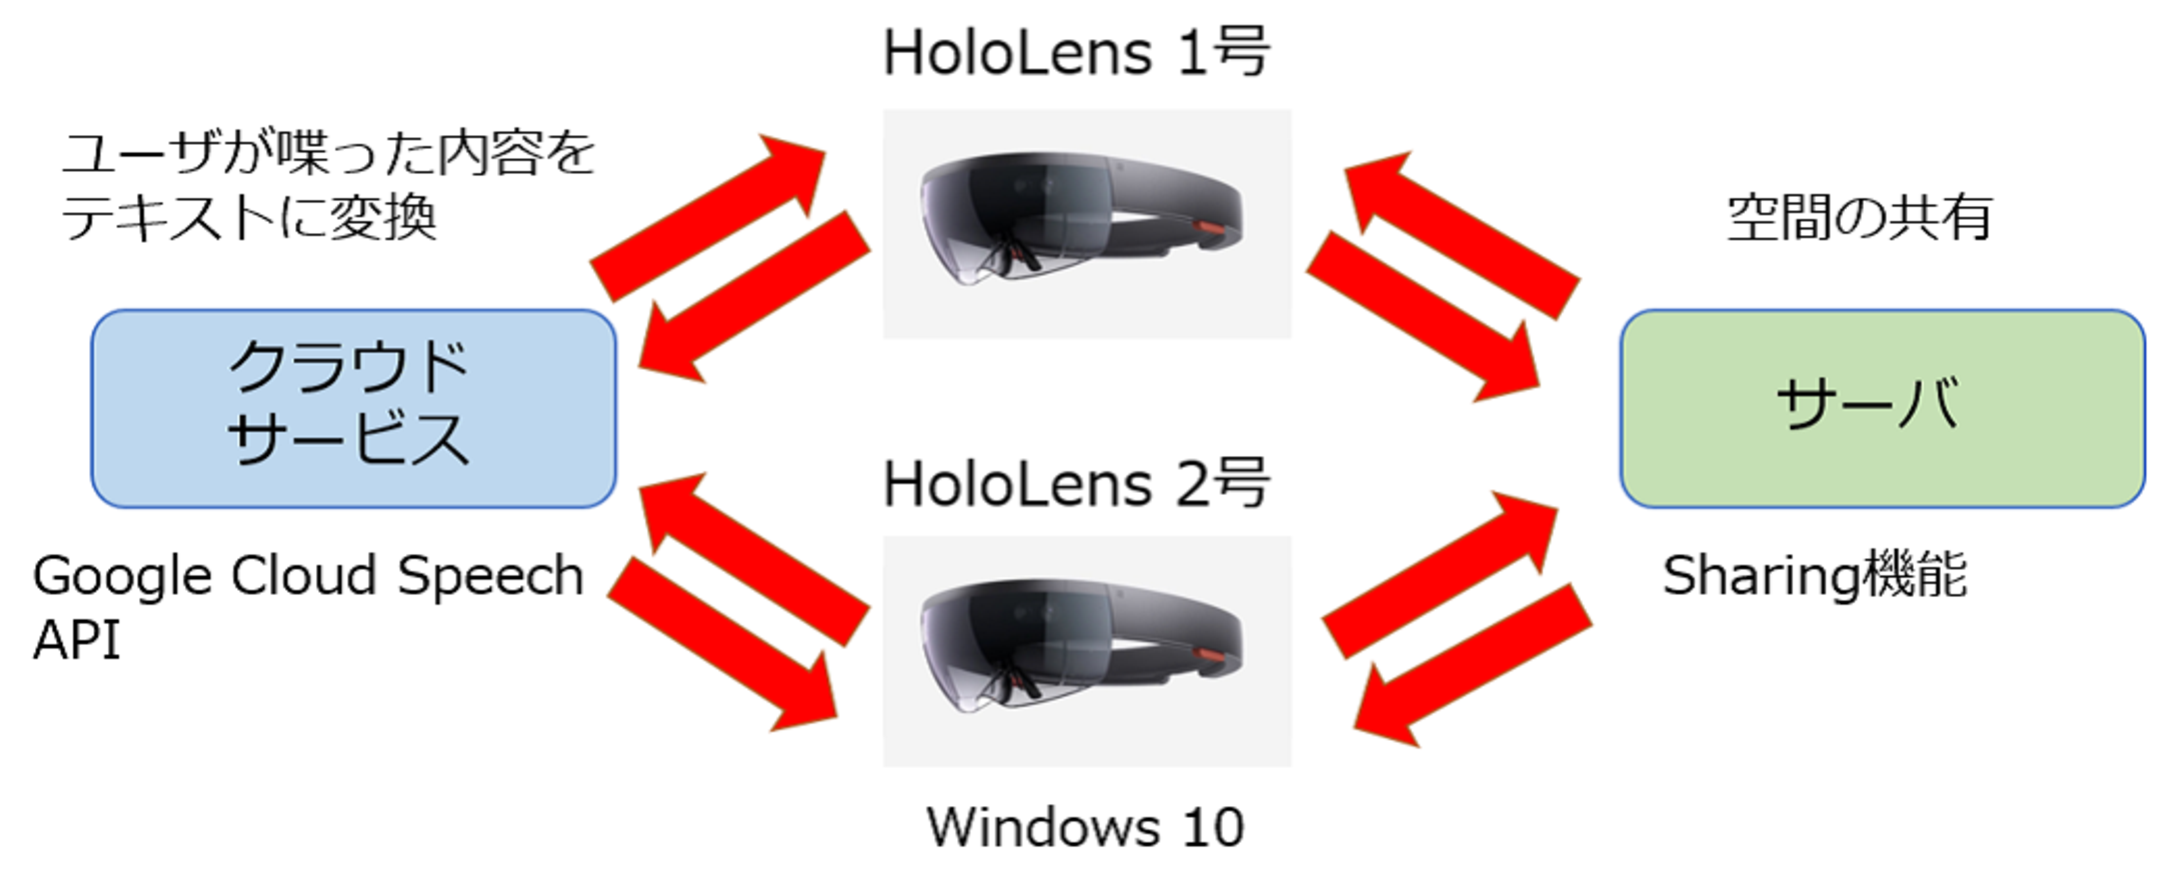
\includegraphics[clip,height=4.0cm,width=9.0cm]{./prototypesystem1.eps}
    \caption{プロトタイプシステムの構成}
    \label{fig:prototypesystem1}
  \end{center}
\end{figure}

\subsubsection{アプリケーション}
Windows 10やWindows 10 Mobile上で動作するUWP(Universal Windows Platform)アプリとして作成すると、HoloLens上でもそのアプリケーションが動作する。アプリケーションの開発には、マイクロソフト社が配布している統合開発環境であるVisual Studio 2017(Ver 15.0)と、ユニティ・テクノロジーズ社が配布している統合開発環境を内蔵した複数のプラットホームに対応するゲームエンジンであるUnity(Ver 5.6.2f1)を使用した。また、Unity 用のHoloLens 向けのツールキットであるHoloToolkit-Unityの導入を行った。開発言語には、Windows向けのアプリケーションの開発に主に使われるC\#を採用した。

\subsubsection{サーバ}
実世界の任意の空間上に残したメモを他のHoloLensを使用している人と共有するには、HoloToolkitのSharingという機能を利用し、Sharing用のサーバを介して空間の共有を行った。HoloLensの座標系は特殊であり、このまま共有をしても現実の空間の同じ位置で物体を共有することはできないという問題が発生する。この問題を解決するためにはアンカーの共有を行った。アンカーとは船の錨の意味で空間内の絶対的な位置に居座ることができるオブジェクトのことである。これを設置することで位置合わせを行い、実世界の任意の空間上に残したメモの共有を行った。

\subsubsection{クラウドサービス}
HoloLensの標準機能で音声入力はサポートされているが、現在利用できる言語が英語のみである。そこでGoogle Cloud Speech APIを利用することにより、日本語の音声をテキストに変換する。Google Cloud Speech APIとはGoogleの持つ音声認識技術を使用し、音声をテキストに変換するサービスである。


%\bibliographystyle{sieicej}
%\bibliography{myrefs}
\begin{thebibliography}{99}% 文献数が10未満の時 {9}
\bibitem{}
\end{thebibliography}

\end{document}
